
\documentclass{IEEEtran}
\usepackage[spanish]{babel}
\usepackage[utf8]{inputenc}
\usepackage{enumerate}
\usepackage{cite}
\usepackage{graphicx}  
\usepackage{subfig}
\usepackage{float}
\usepackage{tikz}
\usepackage{pgfplots}
\usetikzlibrary{pgfplots.dateplot}
\usepackage{pgfplotstable}
\usepackage{filecontents}

% correct bad hyphenation here
\hyphenation{op-tical net-works semi-conduc-tor}


\begin{document}
%
% paper title
% can use linebreaks \\ within to get better formatting as desired
% Do not put math or special symbols in the title.
\title{Práctica 2: Efecto difuminado usando OpenMP}


% author names and affiliations
% use a multiple column layout for up to three different
% affiliations
\author{\IEEEauthorblockN{Andrés Fernando Román Arévalo, Ronald Alexander Sarmiento\\}
\IEEEauthorblockA{Email:afromana@unal.edu.co, roasarmientoga@unal.edu.co\\}
\IEEEauthorblockA{Universidad Nacional Bogotá, Colombia \\}
}


% make the title area
\maketitle

\begin{figure}[!t]
\centering

\includegraphics[width=2.5in]{logo_unal}
\label{fig_sim}
\end{figure}
% As a general rule, do not put math, special symbols or citations
% in the abstract
\begin{abstract}
El siguiente informe presenta como se llevo a cabo la paralelización
 mediante el uso de la interfaz de programación openMP 
 del efecto borroso y los resultados que se obtuvieron tanto de
 Speed Up como de Time Response para los distintas resoluciones
 de imagenes (720p, 1080p y 4k), hilos(1, 2, 4, 8 y 16) y kernels 
 (4, 6, 8, 10, 12 y 14).
\end{abstract}

% no keywords


\IEEEpeerreviewmaketitle



\section{Introducción.}
% no \IEEEPARstart
Una de las tareas altamente demandada en la actualidad 
es el procesamiento de imagenes cada vez de una mayor 
resolución para lo cual se requiere un alto nivel de computo.
 A partir de esto han surgido innumerables algoritmos que permiten
  paralelizar las distintas operaciones del procesamiento de 
  imagenes como lo es la del efecto difuminado.\\

Aun asi paralelizar tiene su limite que es explicado en la 
Ley de Amdahl, la cual establece que hay un punto en que 
paralelizar ya no ofrece mejoras significativas de rendimiento
 e incluso por el contrario puede llevar al deterioro del mismo.\\

Al momento de hacer procesamiento de imagenes se utiliza distintas 
operaciones matriciales.En el caso del efecto borroso se realiza 
una convolucion entre la matriz que representa la imagen y el kernel.

\begin{figure}[H]
  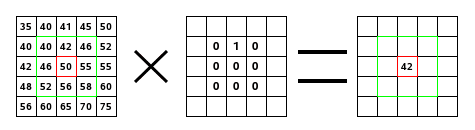
\includegraphics[width=\linewidth]{matriz.png}
  \caption{Convolucion matricial}
  \label{fig:boat1}
\end{figure}
\subsection{Creacion del efecto difuminado}

Se utilizó la tecnica de difuminado conocida 
como Blur el cual consiste en intercambiar cada pixel de la imagen 
por un promedio de los valores RGB que se encuentras en los pixeles 
adyacentes a el. El nivel de difuminado esta determinado por el 
kernel y el tamaño da el rango que se toma para evaluar el promedio.
 Es decir, si se escoge un kernel de 5 significa que cada pixel sera
  cambiado por el prmedio que hay en los promedios de la matriz 5x5
   cuyo centro es el pixel en cuestion.

\section{Paralelización del algoritmo}
La paralelizacion se realizo mediante asignación tipo block-wise
 es decir que se tomo la imagen y se dividio a lo ancho en columnas
  y cada una de estas se asigno a un hilo. 
Asi, para un caso hipotetico donde se quiera aplicar el efecto 
difuminado a una imagen con un ancho de 700 pixeles de ancho,se lanzan 4
 hilos donde el hilo 1 se le asigna la columna 1(del pixel 0 al 175), 
 al 2 la columna 2(del pixel 176 al 350 ), al 3 la columna 3(del 
 pixel 351 al 525)  y al 4 la  columna 4(del pixel 326 al 700). 
 De esta manera, cada hilo tiene para procesar una imagen de
 $(width/THREADS) x \ height$ como se muestra en
  la Figura \ref{paralelizacion}.

\begin{figure}[H]
  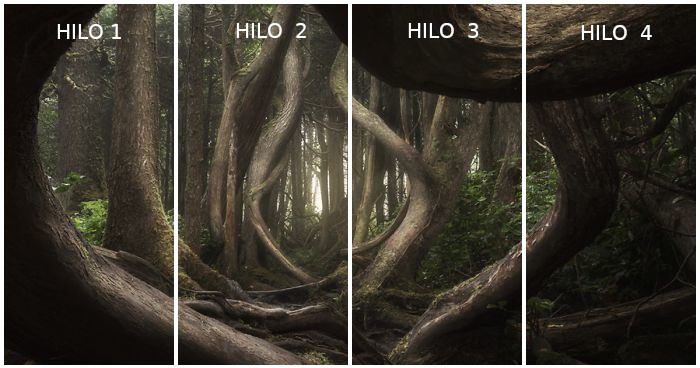
\includegraphics[width=\linewidth]{modi.jpg}
  \caption{Algoritmo de paralelización}
  \label{paralelizacion}
\end{figure}

\section{Experimentos y resultados.}
Antes de mostrar los resultados obtenidos y compararlos con 
los que se obtuvieron al paralelizar el efecto difuso con POSIX, 
es necesario dar a conocer las especificaciones correspondientes 
del ordenador donde corrio el algoritmo. Para esto se construyo 
la siguiente tabla resumiendo dicha información:

\begin{table}[H]
\centering
    \begin{tabular}{ |c|c| } 
\hline
\multicolumn{2}{|c|}{Especificaciones} \\
\hline
Modelo & Lenovo G50-45\\
 \hline
 Procesador & AMD A8-6410 / 2 Gz \\ 
 \hline
 Tarjeta gráfica & AMD Radeon R5 \\ 
 \hline
 Nucleos & 4\\ 
 \hline
 Memoria Ram & 8192 MB DDR3
 \\ 
 \hline
 Sistema operativo & Manjaro 18.0.4 \\ 
 \hline
\end{tabular}
\caption{Especificaciones del ordenador}
\end{table}

Para evitar o disminuir posibles interferencias se corrió
 un script que automaticamente tomó todos los casos de prueba
 mencionados en el resumen, tambien se busco que no hubiese ninguna 
  aplicacion abierta mientras se corria el script.

\subsection{Resultados}
Como primera medida se utilizo el time response o tiempo de 
ejecución de un programa, donde para cada imagen se crearon 
sus corresponientes gráficas donde en eje horizontal se colocaron 
el numero de hilos que ejecutaba el programa y en el eje vertical 
el tiempo que tardo. Para no sobrecargar la gráfica se decidio 
incluir solo tres nucleos por gráfico, eso hace que por resolucion 
de imagen se crearan 2 graficos.\\
A continuacion se presentan las gráficas correspondientes:\\

\begin{itemize}
    \item \textbf{Imagen de 720p}


\begin{tikzpicture}
\begin{axis}[
xticklabels={},
extra x ticks={1,2,4,8,16},
title={Time Response 720p},
xlabel={Numero de hilos},
ylabel={Tiempo},
nodes near coords, 
 every node near coord/.append style={font=\tiny,yshift=-1.6pt},
 nodes near coords style={/pgf/number format/.cd,precision=3},
]
\addplot coordinates { (1,0.28) (2,0.242) (4,0.213) (8,0.216) (16,0.196)  };
\addplot coordinates { (1,0.450) (2,0.294) (4,0.242) (8,0.248) (16,0.245)  };
\addplot coordinates { (1,0.620) (2,0.397) (4,0.301) (8,0.306) (16,0.307)  };
\addlegendentry{Kernel 4}
\addlegendentry{Kernel 6}
\addlegendentry{Kernel 8}
\end{axis}
\end{tikzpicture}

\begin{tikzpicture}
\begin{axis}[
xticklabels={},
extra x ticks={1,2,4,8,16},
title={Time Response 720p},
xlabel={Numero de hilos},
ylabel={Tiempo},
nodes near coords, 
 every node near coord/.append style={font=\tiny,yshift=-1.6pt},
 nodes near coords style={/pgf/number format/.cd,precision=3},
]
\addplot coordinates { (1,0.850) (2,0.525) (4,0.392) (8,0.373) (16,0.382)  };
\addplot coordinates { (1,1.120) (2,0.666) (4,0.453) (8,0.464) (16,0.454)  };
\addplot coordinates { (1,1.558) (2,0.833) (4,0.577) (8,0.554) (16,0.559)  };
\addlegendentry{Kernel 10}
\addlegendentry{Kernel 12}
\addlegendentry{Kernel 14}
\end{axis}
\end{tikzpicture}

\item \textbf{Imagen de 1080p}



\begin{tikzpicture}
\begin{axis}[
xticklabels={},
extra x ticks={1,2,4,8,16},
title={Time Response 1080p},
xlabel={Numero de hilos},
ylabel={Tiempo},
nodes near coords, 
 every node near coord/.append style={font=\tiny,yshift=-1.6pt},
 nodes near coords style={/pgf/number format/.cd,precision=3},
]
\addplot coordinates { (1,0.539) (2,0.385) (4,0.292) (8,0.303) (16,0.310)  };
\addplot coordinates { (1,0.895) (2,0.543) (4,0.392) (8,0.393) (16,0.394)  };
\addplot coordinates { (1,1.34) (2,0.763) (4,0.566) (8,0.523) (16,0.545)  };
\addlegendentry{Kernel 4}
\addlegendentry{Kernel 6}
\addlegendentry{Kernel 8}
\end{axis}
\end{tikzpicture}

\begin{tikzpicture}
\begin{axis}[
xticklabels={},
extra x ticks={1,2,4,8,16},
title={Time Response 1080p},
xlabel={Numero de hilos},
ylabel={Tiempo},
nodes near coords, 
 every node near coord/.append style={font=\tiny,yshift=-1.6pt},
 nodes near coords style={/pgf/number format/.cd,precision=3},
]
\addplot coordinates { (1,1.954) (2,1.105) (4,0.698) (8,0.705) (16,0.729)  };
\addplot coordinates { (1,2.699) (2,1.515) (4,0.954) (8,0.924) (16,0.913)  };
\addplot coordinates { (1,3.587) (2,1.956) (4,1.192) (8,1.214) (16,1.223)  };
\addlegendentry{Kernel 10}
\addlegendentry{Kernel 12}
\addlegendentry{Kernel 14}
\end{axis}
\end{tikzpicture}

\item \textbf{Imagen de 4k}

\begin{tikzpicture}
\begin{axis}[
xticklabels={},
extra x ticks={1,2,4,8,16},
title={Time Response 4k},
xlabel={Numero de hilos},
ylabel={Tiempo},
nodes near coords, 
 every node near coord/.append style={font=\tiny,yshift=-1.6pt},
 nodes near coords style={/pgf/number format/.cd,precision=3},
]
\addplot coordinates { (1,4.941) (2,2.859) (4,2.245) (8,2.190) (16,2.275)  };
\addplot coordinates { (1,9.273) (2,5.134) (4,3.574) (8,3.536) (16,3.587)  };
\addplot coordinates { (1,15.19) (2,8.295) (4,5.436) (8,5.330) (16,5.370)  };
\addlegendentry{Kernel 4}
\addlegendentry{Kernel 6}
\addlegendentry{Kernel 8}
\end{axis}
\end{tikzpicture}

\begin{tikzpicture}
\begin{axis}[
xticklabels={},
extra x ticks={1,2,4,8,16},
title={Time Response 4k},
xlabel={Numero de hilos},
ylabel={Tiempo},
nodes near coords, 
 every node near coord/.append style={font=\tiny,yshift=-1.6pt},
 nodes near coords style={/pgf/number format/.cd,precision=3},
]
\addplot coordinates { (1,22.896) (2,12.262) (4,7.750) (8,7.683) (16,7.711)  };
\addplot coordinates { (1,32.137) (2,17.204) (4,10.662) (8,10.520) (16,10.426)  };
\addplot coordinates { (1,43.849) (2,23.408) (4,14.281) (8,13.948) (16,13.842)  };
\addlegendentry{Kernel 10}
\addlegendentry{Kernel 12}
\addlegendentry{Kernel 14}
\end{axis}
\end{tikzpicture}

\end{itemize}

Como se puede observar en las gráficas anteriores el time response del código tiene cierta tendencia de  mejorar conforme se aumenta la cantidad de hilos que son lanzados hasta los 4 hilos, de ahi en adelante la mejora es insignificante y en algunos casos como en la imagen de 720p se ve cierta desmejora.\\

Otra medida que se considero determinar para medir el rendimiento de los hilos en el programa es el speed up es decir el tiempo de ejecución secuencial dividido entre el tiempo de ejecución por cada una de las cantidad de hilos(1,2,4,8,16). \\
A continuación se presentan las gráficas correspondientes:

\begin{itemize}

\item \textbf{Imagen de 720p}

\begin{tikzpicture}
\begin{axis}[
xticklabels={},
extra x ticks={1,2,4,8,16},
title={Speed Up 720p},
xlabel={Numero de hilos},
ylabel={Speed Up},
nodes near coords, 
 every node near coord/.append style={font=\tiny,yshift=-1.6pt},
 nodes near coords style={/pgf/number format/.cd,precision=3},
 legend pos=south east,
]
\addplot coordinates { (1,1) (2,1.198347107) (4,1.361502347) (8,1.342592593) (16,1.479591837)  };
\addplot coordinates { (1,1) (2,1.530612245) (4,1.859504132) (8,1.814516129) (16,1.836734694)  };
\addplot coordinates { (1,1) (2,1.561712846) (4,2.059800664) (8,2.026143791) (16,2.019543974)  };
\addlegendentry{Kernel 4}
\addlegendentry{Kernel 6}
\addlegendentry{Kernel 8}
\end{axis}
\end{tikzpicture}

\begin{tikzpicture}
\begin{axis}[
xticklabels={},
extra x ticks={1,2,4,8,16},
title={Speed Up 720p},
xlabel={Numero de hilos},
ylabel={Speed Up},
nodes near coords, 
 every node near coord/.append style={font=\tiny,yshift=-1.6pt},
 nodes near coords style={/pgf/number format/.cd,precision=3},
 legend pos=south east,
]
\addplot coordinates { (1,1) (2,1.619047619) (4,2.168367347) (8,2.278820375) (16,2.22513089)  };
\addplot coordinates { (1,1) (2,1.681681682) (4,2.472406181) (8,2.413793103) (16,2.466960352)  };
\addplot coordinates { (1,1) (2,1.870348139) (4,2.70017331) (8,2.812274368) (16,2.787119857)  };
\addlegendentry{Kernel 10}
\addlegendentry{Kernel 12}
\addlegendentry{Kernel 14}
\end{axis}
\end{tikzpicture}

    \item \textbf{Imagen de 1080p}
    
\begin{tikzpicture}
\begin{axis}[
xticklabels={},
extra x ticks={1,2,4,8,16},
title={Speed Up 1080p},
xlabel={Numero de hilos},
ylabel={Speed Up},
nodes near coords, 
 every node near coord/.append style={font=\tiny,yshift=-1.6pt},
 nodes near coords style={/pgf/number format/.cd,precision=3},
 legend pos=south east,
]
\addplot coordinates { (1,1) (2,1.4) (4,1.845890411) (8,1.778877888) (16,1.738709677)  };
\addplot coordinates { (1,1) (2,1.64825046) (4,2.283163265) (8,2.27735369) (16,2.271573604)  };
\addplot coordinates { (1,1) (2,1.756225426) (4,2.367491166) (8,2.562141491) (16,2.458715596)  };
\addlegendentry{Kernel 4}
\addlegendentry{Kernel 6}
\addlegendentry{Kernel 8}
\end{axis}
\end{tikzpicture}
\\
Para estas últimas tre gráficas se decidio omitir a proposito la leyenda del tiempo en cada uno de los nodos, debido a la superposicion que se genera.

\begin{tikzpicture}
\begin{axis}[
xticklabels={},
extra x ticks={1,2,4,8,16},
title={Speed Up 1080p},
xlabel={Numero de hilos},
ylabel={Speed Up},
 legend pos=south east,
]
\addplot coordinates { (1,1) (2,1.768325792) (4,2.799426934) (8,2.771631206) (16,2.680384088)  };
\addplot coordinates { (1,1) (2,1.781518152) (4,2.829140461) (8,2.920995671) (16,2.95618839)  };
\addplot coordinates { (1,1) (2,1.833844581) (4,3.009228188) (8,2.954695222) (16,2.932951758)  };
\addlegendentry{Kernel 10}
\addlegendentry{Kernel 12}
\addlegendentry{Kernel 14}
\end{axis}
\end{tikzpicture}
    
\item \textbf{Imagen de 4k}\\
\begin{tikzpicture}
\begin{axis}[
xticklabels={},
extra x ticks={1,2,4,8,16},
title={Speed Up 4k},
xlabel={Numero de hilos},
ylabel={Tiempo},
 legend pos=south east,
]
\addplot coordinates { (1,1) (2,1.728226653) (4,2.200890869) (8,2.256164384) (16,2.171868132)  };
\addplot coordinates { (1,1) (2,1.806194001) (4,2.594571908) (8,2.622454751) (16,2.585168665)  };
\addplot coordinates { (1,1) (2,1.831223629) (4,2.794334069) (8,2.849906191) (16,2.82867784)  };
\addlegendentry{Kernel 4}
\addlegendentry{Kernel 6}
\addlegendentry{Kernel 8}
\end{axis}
\end{tikzpicture}

\begin{tikzpicture}
\begin{axis}[
xticklabels={},
extra x ticks={1,2,4,8,16},
title={Speed Up 4k},
xlabel={Numero de hilos},
ylabel={Tiempo},
 legend pos=south east
]
\addplot coordinates { (1,1) (2,1.867232099) (4,2.954322581) (8,2.980085904) (16,2.969264687)  };
\addplot coordinates { (1,1) (2,1.867995815) (4,3.014162446) (8,3.054847909) (16,3.082390178)  };
\addplot coordinates { (1,1) (2,1.873248462) (4,3.070443246) (8,3.143748208) (16,3.167822569)  };
\addlegendentry{Kernel 10}
\addlegendentry{Kernel 12}
\addlegendentry{Kernel 14}
\end{axis}
\end{tikzpicture}
    
    
\end{itemize}

Como podemos observar en las gráficas anteriores el speed up es el esperado ya que el tiempo tiene una tendencia a aumentar conforme el programa se ejecuta con más hilos.\\

Por último se consideró importante realizar una comparación de time response entre el código de difuminado usando POSIX 
(descrito en la primera practica) y el actual que es usando la libreria OpenMP. Para simplificar un poco el informe se considero solamente comparar con los kernel 6 y 12 en cada una de las resoluciones de imagen. A continuación se presentan las gráficas correspondientes:\\\\
Para estas ultimas gráficas tambien se decidio omitir la leyenda del tiempo en cada uno de los nodos, debido a la superposición que se genera.

\begin{itemize}
    \item \textbf{Imagen de 720p}
    
    \begin{tikzpicture}
\begin{axis}[
xticklabels={},
extra x ticks={1,2,4,8,16},
title={Time Response 720p},
xlabel={Numero de hilos},
ylabel={Tiempo},
]
\addplot coordinates { (1,0.450) (2,0.294) (4,0.242) (8,0.248) (16,0.245)  };
\addplot coordinates { (1,0.46) (2,0.344) (4,0.260) (8,0.262) (16,0.258)  };
\addplot coordinates { (1,1.120) (2,0.666) (4,0.453) (8,0.464) (16,0.454)  };
\addplot coordinates { (1,1.138) (2,0.691) (4,0.476) (8,0.467) (16,0.465)  };
\addlegendentry{Kernel 6 OpenMP}
\addlegendentry{Kernel 6 POSIX}

\addlegendentry{Kernel 12 OpenMP}
\addlegendentry{Kernel 12 POSIX}
\end{axis}
\end{tikzpicture}

    
\item \textbf{Imagen de 1080p}


\begin{tikzpicture}
\begin{axis}[
xticklabels={},
extra x ticks={1,2,4,8,16},
title={Time Response 1080p},
xlabel={Numero de hilos},
ylabel={Tiempo},
]
\addplot coordinates { (1,0.895) (2,0.543) (4,0.392) (8,0.393) (16,0.394)  };
\addplot coordinates { (1,0.937) (2,0.574) (4,0.408) (8,0.390) (16,0.411)  };
\addplot coordinates { (1,2.699) (2,1.515) (4,0.954) (8,0.924) (16,0.913)  };
\addplot coordinates { (1,2.709) (2,1.512) (4,0.965) (8,0.929) (16,0.944)  };
\addlegendentry{Kernel 6 OpenMP}
\addlegendentry{Kernel 6 POSIX}
\addlegendentry{Kernel 12 OpenMP}
\addlegendentry{Kernel 12 POSIX}
\end{axis}
\end{tikzpicture}


\item \textbf{Imagen de 4k}

\begin{tikzpicture}
\begin{axis}[
xticklabels={},
extra x ticks={1,2,4,8,16},
title={Time Response 4k},
xlabel={Numero de hilos},
ylabel={Tiempo},
]
\addplot coordinates { (1,9.273) (2,5.134) (4,3.574) (8,3.536) (16,3.587)  };
\addplot coordinates { (1,9.306) (2,5.169) (4,3.519) (8,3.576) (16,3.561)  };
\addplot coordinates { (1,32.137) (2,17.204) (4,10.662) (8,10.520) (16,10.426)  };
\addplot coordinates { (1,32.182) (2,17.180) (4,10.654) (8,10.556) (16,10.418)  };
\addlegendentry{Kernel 6 OpenMP}
\addlegendentry{Kernel 6 POSIX}
\addlegendentry{Kernel 12 OpenMP}
\addlegendentry{Kernel 12 POSIX}
\end{axis}
\end{tikzpicture}


\end{itemize}

Como se puede observar en las gráficas existe cierta mejora usando el equivalente de POSIX en OpenMp, aunque esta mejora es más evidente en resolución de imagenes pequeñas como la de 720p.\\
La siguientes tablas ilustran lo anteriormente mencionado:\\
\begin{table}[H]
\centering
    \begin{tabular}{ |c|c|c| } 
\hline
\multicolumn{3}{|c|}{\textbf{Diferencias entre POSIX Y OpenMP}} \\
\hline
\textbf{Hilos} & \textbf{Kernel 6} & \textbf{Kernel 12}\\
\hline
1 Hilo & 0,010 & 0,018\\
 \hline
2 Hilos & 0,050 & 0,025 \\ 
 \hline
4 Hilos & 0,018 & 0,023 \\ 
 \hline
8 Hilos & 0,014 & 0,003\\ 
 \hline
16 Hilos & 0,013 & 0,011\\ 
\hline
\textbf{Promedio de diferencias} & 0,021 & 0,016\\ 
\hline
\end{tabular}
\caption{Imagen de 720p}
\end{table}

\begin{table}[H]
\centering
    \begin{tabular}{ |c|c|c| } 
\hline
\multicolumn{3}{|c|}{\textbf{Diferencias entre POSIX Y OpenMP}} \\
\hline
\textbf{Hilos} & \textbf{Kernel 6} & \textbf{Kernel 12}\\
\hline
1 Hilo & 0,042 & 0,01\\
 \hline
2 Hilos & 0,031 & -0,003 \\ 
 \hline
4 Hilos & 0,016 & 0,011 \\ 
 \hline
8 Hilos & -0,003 & 0,005\\ 
 \hline
16 Hilos & 0,017 & 0,031\\ 
\hline
\textbf{Promedio de diferencias} & 0,0206 & 0,0108\\ 
\hline
\end{tabular}
\caption{Imagen de 1080p}
\end{table}

\begin{table}[H]
\centering
    \begin{tabular}{ |c|c|c| } 
\hline
\multicolumn{3}{|c|}{\textbf{Diferencias entre POSIX Y OpenMP}} \\
\hline
\textbf{Hilos} & \textbf{Kernel 6} & \textbf{Kernel 12}\\
\hline
1 Hilo & 0,042 & 0,01\\
 \hline
2 Hilos & 0,035 & -0,024 \\ 
 \hline
4 Hilos & -0,055 & 0,011 \\ 
 \hline
8 Hilos & 0,040 & 0,036\\ 
 \hline
16 Hilos & -0,026 & -0,008\\ 
\hline
\textbf{Promedio de diferencias} & 0,0054 & 0,0082\\ 
\hline
\end{tabular}
\caption{Imagen de 4k}
\end{table}

Con base en los datos tabulados se  calculó la diferencia promedio entre la ejecución de POSIX y OpenMP en la paralelización del efecto difuminado. Para los kernel de 6 y 12 en el caso de la imagen de 720p es de 0,0185 segundos, en el caso de la imagen de 1080p es de 0,0157 segundos y en el caso de la imagen de 4k es de 0,0068 segundos. Por último cabe mencionar que la diferencia promedio global es de 0,01366666667 segundos.

\section*{Conclusiones.}
\begin{itemize}
  \item Cuanto mas grande es el kernel con el que se trabaja se tarda un tiempo superior en realizar el efecto difuminado debido a que realiza mas operaciones al momento de calcular el promedio del kernel, haciendo que el costo computacional sea superior.
  \item Como se observa en los resultados presentados en las tablas anteriores la mejora solo se aprecia que es significativa hasta los 4 hilos y considero que se debe a que el procesador donde se corrio el código  solo posee 4 núcleos
  \item Aunque la diferencia entre el uso de POSIX y OpenMP podria parecer muy pequeña en realidad al momento de hacer un gran conjunto de  operaciónes que requieran de un cómputo mas prolongado los tiempos tenderán a escalar.
  \item Cabe mencionar que la implementación de OpenMP es muy sencilla incluso cuando el programa es secuencial, lo que va a permitir migrar a una computacion paralela rápidamente cuando existe alta densidad de código.
\end{itemize}


\noindent 


\begin{thebibliography}{00}
\bibitem{b2} Pedraza, C. (2019). Diapositivas de clase.
\bibitem{b1}David, K. and Wen-Mei, H. (2010). Programming massively parallel processos. 2nd ed. Morgan Kaufmann.
\bibitem{b2} Thomas, R. and Gudula, R. (2010). Parallel Programming. 1st ed. Springer.
\bibitem{b2} En.wikipedia.org. $(2019). Box blur.  Available at: https://en.wikipedia.org/wiki/Box_blur.$
\end{thebibliography}




% that's all folks
\end{document}


